\documentclass{standalone}
\usepackage{tikz}
\usepackage{ctex,siunitx}
\setCJKmainfont{Noto Serif CJK SC}
\usepackage{tkz-euclide}
\usepackage{amsmath}
\usetikzlibrary{patterns, calc,3d}
\usetikzlibrary {decorations.pathmorphing,decorations.pathreplacing,decorations.shapes}
\begin{document}
\small
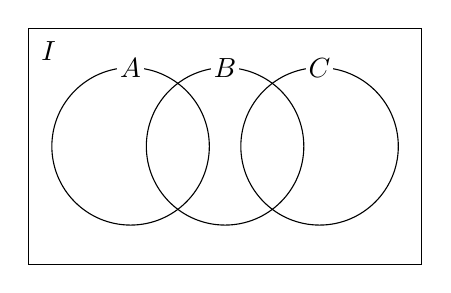
\begin{tikzpicture}[>=latex,scale=1.0,inner sep=1pt]
  \draw(0,0)circle(1);
  \draw(1.2,0)circle(1);
  \draw(-1.2,0)circle(1);
  \draw (-2.5,1.5)node[below right=5pt]{$I$}rectangle(2.5,-1.5);
  \node at (-1.2,1)[fill=white]{$A$};
  \node at (0,1)[fill=white]{$B$};
  \node at (1.2,1)[fill=white]{$C$};
\end{tikzpicture}
\end{document}